\documentclass[11pt]{article}
\usepackage{tikz} 
\usepackage{times}
\usepackage{palatino}
\usepackage{forest}
\usepackage[colorlinks=true, linkcolor=cyan, urlcolor=cyan, citecolor=cyan]{hyperref} % 超链接
\usepackage{pgfplots} % 绘图
\pgfplotsset{compat=newest} % 绘图兼容模式
\usepackage{enumitem}
\usepackage{amssymb}
\usepackage{amsmath}
\usepackage{listings}
\usepackage{xcolor}
\usepackage{palatino}
\usepackage{algorithm}
\usepackage{algpseudocode}
\usepackage{comment}
\usepackage{graphicx} 
\setlength{\parindent}{0pt}

% template styling
\oddsidemargin=-0.005in
\evensidemargin=-0.005in
\textwidth=6.50in
\textheight=9.0in
\topmargin=-0.5in
\setlength{\parindent}{0pt} % zero indent
\newenvironment{tempspacing}[1]{\begin{trivlist}
\baselineskip=#1
\normalbaselineskip=\baselineskip\item[]}{\end{trivlist}}
\renewcommand{\baselinestretch} {1.2}
\pagenumbering{arabic}
\pagestyle{empty}
\thispagestyle{empty}

\begin{document}

%%% Frontmatter %%%
\title{\large\bf \vspace*{-0.3in}CSE 6220 High Performance Computing\\
Programming Assignment-3 Report \\Submitted \today}
\author{}
\date{}
\maketitle
\vspace*{-0.8in}
{\bf Name:} Honglin Liu \hfill{{\bf gID:} 903651409}\\
{\bf Name:} Xuzheng Tian \hfill{{\bf gID:} 903618682}\\

%%% Main text %%%
\section{Implementation of the 2D SUMMA SpGeMM Algorithm}

Our implementation of the Sparse General Matrix-Matrix Multiplication (SpGeMM) algorithm computes $C = A \times B$ for sparse matrices $A$ ($m \times p$) and $B$ ($p \times n$) in COO (Coordinate List Format) format, using a 2D $\sqrt{p} \times \sqrt{p}$ processor grid. 

We adopt the Sparse \href{https://www.netlib.org/lapack/lawnspdf/lawn96.pdf}{SUMMA} (Scalable Universal Matrix Multiplication) algorithm, optimized for non-zero elements, with key functions implemented in \texttt{SpGeMM.cpp}.

\subsection{Algorithm implementation}
The algorithm proceeds as follows:
\begin{enumerate}
	\item \textbf{Initialization}:\\
        {\color{blue}The root processor distributes input matrices $A$ and $B$ in global COO format to the $\sqrt{p} \times \sqrt{p}$ processor grid, with each processor receiving entries for its block without coordinate adjustments. }\\
        The \texttt{SpGeMM\_2d} function determines the local block dimensions for each processor.\\
        A local matrix \texttt{C\_block} is created as a sparse map, with elements implicitly set to 0 (non-existent entries are treated as 0 during computation). \\
        
    \item \textbf{COO to CSR Conversion}:\\
        To optimize non-zero element access, \texttt{COO2CSR} converts input matrices $A$ and $B$ from COO to CSR (Compressed Sparse Row) format.\\
        For a matrix with \texttt{lenth} non-zeros, \texttt{COO2CSR} allocates \texttt{row\_ptr} (size \texttt{m+1}), \texttt{idx}, and \texttt{values} (size \texttt{lenth}).\\
        It counts non-zeros per row and computes a prefix sum for \texttt{row\_ptr}, enabling efficient row-wise traversal.

    \item \textbf{SUMMA Computation}:\\
        The \texttt{SUMMA} function executes the core multiplication.\\
        For each iteration $k$ (0 to $\sqrt{P}$):
    \begin{itemize}[topsep=0pt, itemsep=0pt]
        \item \textbf{Broadcast $A$}:\\ 
            The $k$-th column block of $A$ (CSR format) is broadcast within the row communicator (\texttt{row\_comm}) using \texttt{MPI\_Bcast}.\\
            The block includes \texttt{row\_ptr}, \texttt{idx}, and \texttt{values}, with size determined by non-zero count (\texttt{nnz\_A}).
        \item \textbf{Broadcast $B$}:\\
            The $k$-th row block of $B$ is broadcast within the column communicator (\texttt{col\_comm}).
        \item \textbf{Local Computation}:\\
            Each processor computes a contribution to $C$’s local block (\texttt{C\_block}, a sparse map of coordinates to values).\\
            For each non-zero $A[i, A\_col]$ and $B[A\_col, B\_col]$, we update \texttt{C\_block[\{i, B\_col\}] = plus(C\_block[\{i, B\_col\}], times(A[i, A\_col], B[A\_col, B\_col]))}, where \texttt{plus} and \texttt{times} define the semiring.
    \end{itemize}
    \texttt{C\_block} is initialized as an empty \texttt{std::map} in \texttt{SpGeMM\_2d}, storing {\color{red} all entries}.

    \item \textbf{Output Conversion}:\\
        The \texttt{MTX2COO} function converts \texttt{C\_block} to COO format.\\
        {\color{blue}It iterates over non-zero entries in the sparse map, using their global coordinates directly to form the output matrix $C$.}
\end{enumerate}

% brief summary
{\color{blue}For APSP, \texttt{SpGeMM\_2d} is used with the min-plus semiring, treating undeclared values in \texttt{C\_block} as infinity and setting diagonal entries to 0 to compute shortest paths correctly.}

The implementation ensures correctness for arbitrary $m \times p$ and $p \times n$ matrices while supporting flexible semiring operations, as tested with $A \times A^T$.

\newpage
\section{Implementation of the APSP Algorithm}

The APSP (All-Pairs Shortest Path) algorithm computes shortest path distances between all vertex pairs in a weighted graph with $n$ nodes, represented in COO format.  

Inspired by the \href{https://en.wikipedia.org/wiki/Floyd\%E2\%80\%93Warshall_algorithm}{\textit{Floyd-Warshall}} algorithm, our implementation in \texttt{apsp.cpp} uses matrix multiplication with a \textit{min-plus} semiring operator, executed via \texttt{SpGeMM\_2d}.  

The graph described in the problem is modeled as an $n \times n$ distance matrix $L$, where $L[i,j]$ is the edge weight from node $i$ to $j$ (0 denotes infinity). 

% semiring operation 
\subsection{Implementation of min-plus semiring}
The \textit{min-plus} semiring redefines operations:
\begin{itemize}[topsep=0pt, itemsep=0pt]
    \item \texttt{plus}:\\
          {\color{blue}$\min(a, b)$, selecting the shorter path. If $a=0$ (infinity), returns $b$; otherwise, returns the minimum of $a$ and $b$.}
    \item \texttt{times}:\\
          {\color{blue}$a + b$, summing edge weights directly, assuming valid weights (zeros as 0).}
\end{itemize}
{\color{blue}This allows $L^k[i,j]$ to represent the shortest path from $i$ to $j$ using at most $k$ intermediate nodes. Diagonal entries are set to 0 after each iteration to ensure correctness.}

% algorithm framework
\subsection{Algorithm implementation}
The algorithm proceeds as follows:
\begin{enumerate}
    \item \textbf{Initialization}:\\
          In \texttt{apsp}, we set $L$ to the input graph and compute local block ranges for each processor (\texttt{row\_rank}, \texttt{col\_rank}) in the $\sqrt{p} \times \sqrt{p}$ grid.\\
          The block size is \texttt{block\_size\_n = (n+row\_size-1)/row\_size}, with row range [\texttt{row\_start}, \texttt{row\_end}) and column range [\texttt{col\_start}, \texttt{col\_end}).

    \item \textbf{Iterative Matrix Multiplication}:\\
        For iterations where \texttt{max\_iter} doubles from 1 to $n$:
        \begin{itemize}[topsep=0pt, itemsep=0pt]
            \item Copy $L$ to \texttt{L\_tmp}.
            \item Call \texttt{SpGeMM\_2d} to compute $L = \texttt{L\_tmp} \times \texttt{L\_tmp}$ under the min-plus semiring, updating $L[i,j] = \min(L[i,j], \min_k (L[i,k] + L[k,j]))$.
            {\color{blue}\item Set diagonal entries $L[i,i]$ to 0 to correct potential errors from summation or minimization.}
        \end{itemize}

    \item \textbf{Local Processing}:\\
          {\color{blue}Each processor retains $L$’s entries in global coordinates, with no additional filtering required beyond diagonal corrections performed in step 2.}

    \item \textbf{Synchronization}:\\
          \texttt{MPI\_Barrier} ensures processors align after each iteration.

    \item \textbf{Output}:\\
          Global coordinates are restored by adding \texttt{row\_start} and \texttt{col\_start} offsets, yielding the result in COO format.
\end{enumerate}

This \href{https://en.wikipedia.org/wiki/Floyd\%E2\%80\%93Warshall_algorithm}{\textit{Floyd-Warshall}}-inspired approach leverages \texttt{SpGeMM\_2d}’s parallel efficiency to compute shortest paths.  
The \textit{min-plus} semiring ensures correctness, while local processing reduces communication overhead.

\newpage
\section{Analysis of Algorithms' Performances}

\begin{comment}
Running with 1 processors
srun: warning: can't run 1 processes on 2 nodes, setting nnodes to 1
==> time_taken=55.6141s
==> SpGeMM_result size=80542131
==> correctness_check=ok
Running with 4 processors
==> time_taken=18.5754s
==> SpGeMM_result size=80542131
==> correctness_check=ok
Running with 9 processors
==> time_taken=10.2716s
==> SpGeMM_result size=80542131
==> correctness_check=ok
Running with 16 processors
==> time_taken=6.97158s
==> SpGeMM_result size=80542131
==> correctness_check=ok
Running with 25 processors
==> time_taken=5.18539s
==> SpGeMM_result size=80542131
==> correctness_check=ok
Running with 36 processors
==> time_taken=4.12954s
==> SpGeMM_result size=80542131
==> correctness_check=ok
-------------------------------------
Running with 49 processors
-------------------------------------
Running with 1 processors
srun: warning: can't run 1 processes on 2 nodes, setting nnodes to 1
==> time_taken=991.476s
==> correctness_check=ok
Running with 4 processors
==> time_taken=188.953s
==> correctness_check=ok
Running with 9 processors
==> time_taken=69.9142s
==> correctness_check=ok
Running with 16 processors
==> time_taken=32.8895s
==> correctness_check=ok
Running with 25 processors
==> time_taken=18.0195s
==> correctness_check=ok
Running with 36 processors
==> time_taken=11.2759s
==> correctness_check=ok
\end{comment}

\begin{comment}
(base) [hliu686@atl1-1-02-012-23-1 code]$ sh autograder.sh
Architecture:             x86_64
  CPU op-mode(s):         32-bit, 64-bit
  Address sizes:          46 bits physical, 48 bits virtual
  Byte Order:             Little Endian
CPU(s):                   24
  On-line CPU(s) list:    0-23
Vendor ID:                GenuineIntel
  Model name:             Intel(R) Xeon(R) Gold 6226 CPU @ 2.70GHz
    CPU family:           6
    Model:                85
    Thread(s) per core:   1
    Core(s) per socket:   12
    Socket(s):            2
    Stepping:             7
    CPU(s) scaling MHz:   73%
    CPU max MHz:          3700.0000
    CPU min MHz:          1200.0000
    BogoMIPS:             5400.00
    Flags:                fpu vme de pse tsc msr pae mce cx8 apic sep mtrr pge mca cmov pat pse36 clflu
                          sh dts acpi mmx fxsr sse sse2 ss ht tm pbe syscall nx pdpe1gb rdtscp lm const
                          ant_tsc art arch_perfmon pebs bts rep_good nopl xtopology nonstop_tsc cpuid a
                          perfmperf pni pclmulqdq dtes64 monitor ds_cpl vmx smx est tm2 ssse3 sdbg fma 
                          cx16 xtpr pdcm pcid dca sse4_1 sse4_2 x2apic movbe popcnt tsc_deadline_timer 
                          aes xsave avx f16c rdrand lahf_lm abm 3dnowprefetch cpuid_fault epb cat_l3 cd
                          p_l3 intel_ppin ssbd mba ibrs ibpb stibp ibrs_enhanced tpr_shadow flexpriorit
                          y ept vpid ept_ad fsgsbase tsc_adjust bmi1 avx2 smep bmi2 erms invpcid cqm mp
                          x rdt_a avx512f avx512dq rdseed adx smap clflushopt clwb intel_pt avx512cd av
                          x512bw avx512vl xsaveopt xsavec xgetbv1 xsaves cqm_llc cqm_occup_llc cqm_mbm_
                          total cqm_mbm_local dtherm ida arat pln pts hwp hwp_act_window hwp_epp hwp_pk
                          g_req vnmi pku ospke avx512_vnni md_clear flush_l1d arch_capabilities
Virtualization features:  
  Virtualization:         VT-x
Caches (sum of all):      
  L1d:                    768 KiB (24 instances)
  L1i:                    768 KiB (24 instances)
  L2:                     24 MiB (24 instances)
  L3:                     38.5 MiB (2 instances)
NUMA:                     
  NUMA node(s):           2
  NUMA node0 CPU(s):      0-11
  NUMA node1 CPU(s):      12-23
Vulnerabilities:          
  Gather data sampling:   Vulnerable
  Itlb multihit:          KVM: Mitigation: VMX disabled
  L1tf:                   Not affected
  Mds:                    Not affected
  Meltdown:               Not affected
  Mmio stale data:        Vulnerable
  Reg file data sampling: Not affected
  Retbleed:               Vulnerable
  Spec rstack overflow:   Not affected
  Spec store bypass:      Vulnerable
  Spectre v1:             Vulnerable: __user pointer sanitization and usercopy barriers only; no swapgs
                           barriers
  Spectre v2:             Vulnerable; IBPB: disabled; STIBP: disabled; PBRSB-eIBRS: Vulnerable; BHI: Vu
                          lnerable
  Srbds:                  Not affected
  Tsx async abort:        Mitigation; TSX disabled

Lmod is automatically replacing "mvapich2/2.3.7-1" with "openmpi/4.1.5".

Due to MODULEPATH changes, the following have been reloaded:
  1) gmp/6.2.1     2) mpc/1.3.1     3) mpfr/4.2.0     4) zlib/1.2.13

rm -f pa3 *.o
mpic++ -O3 -Wall -c SpGeMM.cpp
mpic++ -O3 -Wall -c apsp.cpp
mpic++ -O3 -Wall -c distribute.cpp
mpic++ -O3 -Wall -c pa3.cpp
mpic++ -O3 -Wall -o pa3 pa3.o SpGeMM.o apsp.o distribute.o
=================== CORRECTNESS TESTS ===================

TESTING SpGeMM:

==> Testing P=1:
====> testfiles/ibm32-SpGeMM.dat: OK
====> testfiles/simple-SpGeMM.dat: OK
==> Testing P=4:
====> testfiles/ibm32-SpGeMM.dat: OK
====> testfiles/simple-SpGeMM.dat: OK
==> Testing P=9:
====> testfiles/ibm32-SpGeMM.dat: OK
====> testfiles/simple-SpGeMM.dat: OK
==> Testing P=16:
====> testfiles/ibm32-SpGeMM.dat: OK
====> testfiles/simple-SpGeMM.dat: OK
==> Testing P=25:
====> testfiles/ibm32-SpGeMM.dat: OK
====> testfiles/simple-SpGeMM.dat: OK
==> Testing P=36:
====> testfiles/ibm32-SpGeMM.dat: OK
====> testfiles/simple-SpGeMM.dat: OK

*************************************
SpGeMM PASSED
-------------------------------------

TESTING APSP:

==> Testing P=1:
====> testfiles/ibm32-apsp.dat: OK
====> testfiles/simple-apsp.dat: OK
==> Testing P=4:
====> testfiles/ibm32-apsp.dat: OK
====> testfiles/simple-apsp.dat: OK
==> Testing P=9:
====> testfiles/ibm32-apsp.dat: OK
====> testfiles/simple-apsp.dat: OK
==> Testing P=16:
====> testfiles/ibm32-apsp.dat: OK
====> testfiles/simple-apsp.dat: OK
==> Testing P=25:
====> testfiles/ibm32-apsp.dat: OK
====> testfiles/simple-apsp.dat: OK
==> Testing P=36:
====> testfiles/ibm32-apsp.dat: OK
====> testfiles/simple-apsp.dat: OK

*************************************
APSP PASSED
-------------------------------------

=================== PERFORMANCE TESTS ===================

TESTING SpGeMM WITH perf-testfiles/GL7d14.dat:

==> Testing P=16:
====> PASSED (runtime of 7.07546s)
==> Testing P=36:
====> PASSED (runtime of 4.19513s)

*************************************
SpGeMM PASSED PERFORMANCE TEST
-------------------------------------

TESTING APSP WITH perf-testfiles/G12.dat:

==> Testing P=16:
====> PASSED (runtime of 33.674s)
==> Testing P=36:
====> PASSED (runtime of 11.978s)

*************************************
APSP PASSED PERFORMANCE TEST
-------------------------------------	
\end{comment}

We analyze the theoretical computational complexity and communication costs;
with PACE clusters, we also record the actual performances of our SpGeMM (\texttt{SpGeMM\_2d}) and APSP (\texttt{apsp}) implementations on a $\sqrt{p} \times \sqrt{p}$ processor grid with $P = 1^2, 2^2, 3^2, 4^2, 5^2, 6^2$.



\subsection{Complexity and Communication}
{\color{blue}
\textbf{SpGeMM}: 
\begin{itemize}[label={},itemsep=0pt,topsep=0pt] 
    \item \textbf{Comput. cost}:\\
        $O((\text{nnz}(A) \cdot \text{nnz}(B))/p + \sqrt{p})$ for one matrix multiplication.  
    \item \textbf{Comm. cost}:\\
        $\sqrt{p}$ \texttt{MPI\_Bcast} calls cost $O(\tau \cdot \sqrt{p} + \mu \cdot (\text{nnz}(A) + \text{nnz}(B))/\sqrt{p})$ per processor
\end{itemize}

\textbf{APSP}:
\begin{itemize}[label={}, itemsep=0pt,topsep=0pt]   
    \item  \textbf{Comput.cost}:\\
        $O((\text{nnz}(G)^2 \cdot \log n)/p + \sqrt{p} \cdot \log n)$ for $\text{nnz}(G)$ edges, due to $\lceil \log n \rceil$ \texttt{SpGeMM\_2d} calls.  
    \item  \textbf{Comm. cost}:\\ 
        $\log n$ $\times$ SpGeMM’s cost $+$ \texttt{MPI\_Barrier}, totaling $O(\tau \cdot \sqrt{p} \cdot \log n + \mu \cdot \text{nnz}(G) \cdot \log n / \sqrt{p})$ per processor.
\end{itemize}
}

*: 
nnz \textit{abbr.} for ``number of non-zero elements'';
$G :=$ Graph;
$\tau$ is latency; 
$\mu$ is bandwidth.
\\[1ex]

{\color{blue}
\textbf{Comparison}:\\
SpGeMM is lighter (single pass) but scales similarly to APSP per iteration. 
APSP’s $\log n$ iterations inflate computation and communication, reducing scalability for large $n$.
}

\subsection{Performance visualization}

\begin{figure}[H]
    \centering
    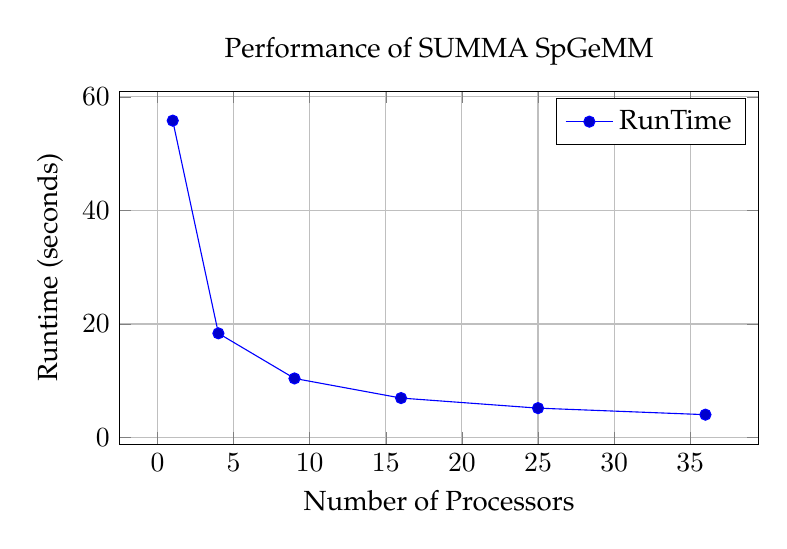
\begin{tikzpicture}
        \begin{axis}[
            width=0.8\textwidth,
            height=0.5\textwidth,
            xlabel={Number of Processors},
            ylabel={Runtime (seconds)},
            title={Performance of SUMMA SpGeMM},
            mark=*,
            grid=major
        ]
        \addplot coordinates {
            (1,  55.8031)
            (4,  18.3599)
            (9,  10.4209)
            (16, 6.96616)
            (25, 5.19271)
            (36, 4.04231)
        };
        \addlegendentry{RunTime}
        \end{axis}
    \end{tikzpicture}
    \caption{\color{blue}SpGeMM: 55.80s to 4.04s ($p=36$, speedup 13.80$\times$).}
\end{figure}

SpGeMM Scales from {\color{blue}55.80s ($p=1$)} to {\color{blue}4.04s ($p=36$)}, meeting $<10$s target. Speedup ({\color{blue}13.80$\times$}) slows beyond $p=16$ due to communication ($O(\alpha \cdot \sqrt{p})$). 
 
\begin{figure}[H]
    \centering
    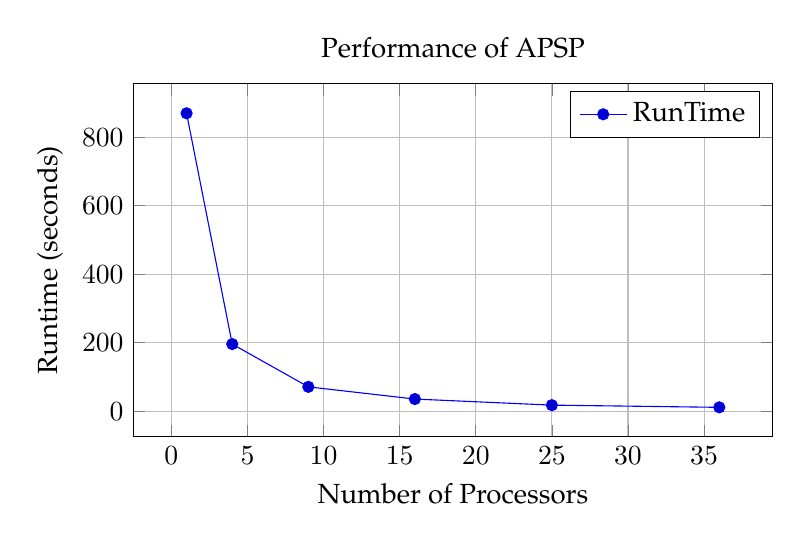
\begin{tikzpicture}
        \begin{axis}[
            width=0.8\textwidth,
            height=0.5\textwidth,
            xlabel={Number of Processors},
            ylabel={Runtime (seconds)},
            title={Performance of APSP},
            mark=*,
            grid=major
        ]
        \addplot coordinates {
            (1,  869.63)
            (4,  195.712)
            (9,  70.8182)
            (16, 35.1929)
            (25, 17.4393)
            (36, 11.0055)
        };
        \addlegendentry{RunTime}
        \end{axis}
    \end{tikzpicture}
    \caption{\color{blue}APSP: 869.63s to 11.01s ($p=36$, speedup 79.02$\times$).}
\end{figure}

APSP Drops from {\color{blue}869.63s} to {\color{blue}11.01s}, exceeding $<30$s target. Higher speedup ({\color{blue}79.02$\times$}) reflects more enormous sequential workload, but $\log n$ iterations limit scalability.\\ 

% Comparison
APSP’s iterative cost yields higher runtimes but better speedup. 
Both face load imbalance and communication bottlenecks at high $p$.

% Summary 

\end{document}
%%% Local Variables:
%%% mode: latex
%%% TeX-master: t
%%% End: